\documentclass{report}
\usepackage[
backend=biber,
style=nature,
]{biblatex}
\addbibresource{references.bib} %Import the bibliography file
\usepackage{graphicx} % Required for inserting images
\usepackage{float}
\usepackage{booktabs}
\usepackage{longtable}
\usepackage{tablefootnote}
\usepackage{caption}
\captionsetup[figure]{font=footnotesize}

%\title{Accelerating sporting expertise through effectice learning problems and teaching signals}
%\title{Making the hours count: can we improve skill learning by using more effective learning problems and more effective teaching signals?}
\title{Skill learning in elite athletes: can we improve skill learning by using more effective learning problems and more effective teaching signals?}


\author{Christian Magelssen}
\date{January 2024}

\begin{document}
\newcommand{\RNum}[1]{\uppercase\expandafter{\romannumeral #1\relax}}

\maketitle

\tableofcontents 
\listoffigures




\chapter{Introduction}

Humans show a remarkable ability to learn new skills, such as driving a car or skiing down an easy slope after just a few hours of practice. But beyond these everyday skills, there also exists an upper level of performance that only the fewest of us attain—such as playing in the Wimbledon tennis finals—and that is achievable only through many years of dedicated practice \cite{hodges_predicting_2004, ericsson_role_1993, vaeyens_talent_2009}. Skill learning can thus be viewed not only as a process of becoming competent but also as one that can be extended to achieve extraordinary skills \cite{ericsson_development_2003, ericsson_scientific_1998}. Understanding how some individuals make the leap from this initial competence to become experts and whether there are learning strategies that may accelerate this transition has long intrigued scientists across various disciplines \cite{ericsson_expert_1994, ericsson_scientific_1998, ericsson_development_2003, ericsson_prospects_2002} and has significant implications for many aspects of life.

In recent decades, cognitive science has made great strides in understanding the mechanisms that likely exert control of skill learning and how they can be leveraged to improve learning and performance \cite{wolpert_principles_2011, makino_circuit_2016, spampinato_multiple_2021, krakauer_motor_2019, haith_model-based_2013, huang_rethinking_2011, shmuelof_are_2011, doya_complementary_2000}. Most of these studies have leaned toward simple, laboratory-based learning tasks\cite{krakauer_motor_2019, du_relationship_2022}, such as button/ball pressing \cite{hardwick_time-dependent_2019, vassiliadis_reward_2021} or reaching movements\cite{shadmehr_adaptive_1994, krakauer_learning_2000},  which enable scientists to dissect and closely examine the contributions of individual learning mechanisms in a controlled environment \cite{spampinato_multiple_2021}. But their advantage also comes with a cost; they are unlikely to capture the full complexity of real-world skill learning \cite{krakauer_motor_2019, mangalam_investigating_2023, du_relationship_2022, chen_effects_2018, wolpert_principles_2011, gallivan_decision-making_2018, iyer_probing_2020, ingram_naturalistic_2011}. Therefore, an outstanding question is whether insights from these studies have brought us closer to understanding and improving the learning of real-world skills, which engage all learning mechanisms simultaneously \cite{spampinato_multiple_2021}. Bridging the gap between laboratory and real-world learning has thus been identified as a critical direction for future research to learn whether these theories have practical applications in natural environments, such as sports, education, and rehabilitation \cite{du_relationship_2022, wolpert_motor_2010, yarrow_inside_2009, haar_motor_2020, ingram_naturalistic_2011}.

Elite sports offer an exciting test domain for these theories because they present one of the most demanding learning challenges for the brain \cite{walsh_is_2014}. First, elite athletes must learn to optimize their performance across many situations and conditions\cite{mangalam_investigating_2023, du_relationship_2022, krakauer_motor_2019}. The need for this adaptability is one reason why achieving elite status requires many years of training \cite{krakauer_motor_2019}, in stark contrast to simpler laboratory tasks where participants reach peak performance after just minutes, hours, or days of training, and researchers already know the best solution. Second, sports involve full-body movements, unlike laboratory tasks, which typically involve only one or a few degrees of freedom \cite{du_relationship_2022}. Finally, sports are not trivial activities but generally hold intrinsic value for athletes, as they constitute an important part of their life. Therefore, athletes are generally motivated to improve their skills. Together, these characteristics make elite sports a unique and compelling domain for testing these learning theories.

Studying skill learning in elite athletes presents its own methodological challenges, however. By definition, elite athletes are already highly skilled and are expected to show minimal improvement by repeating their automated solution with additional training\cite{ericsson_development_2003, ericsson_expert_1994, ericsson_scientific_1998}. Consequently, learning experiments targeting familiar solutions are unlikely to bring improvement in performance, making elite sports an unsuitable domain for studying skill learning processes  \cite{thorndike_educational_1913, ericsson_development_2003, grayloooooong, grayshort, ericsson_scientific_1998}. However, this obstacle can be overcomed by rethinking the approach taking to the learning experiments. Often, the reason elite athletes do not progress is their lack of knowledge about better methods to solve tasks \cite{grayloooooong, grayshort, thorndike_educational_1913}. Therefore, developing strategies that help athletes improve task performance could significantly enhance their skills and is essential for testing learning theories on this skilled cohort of athletes. 
%However, this lack of improvement does not mean skilled performers cannot improve. Often, their limited performance improvement reflects a plateau caused by a lack of knowledge about better methods to solve the task. Helping athletes discover better strategies can enable them to overcome these limits and ensure performance advancement. Therefore, a necessary condition for conducting learning experiments with skilled athletes is finding ways to make them improve their skill.

Due to the necessity of finding ways to improve elite athletes' skills, this doctoral project has two overarching goals. On the one hand, it seeks to identify areas where elite athletes can improve and build knowledge and understanding of strategies they can use to achieve this. On the other hand, it aims to use this knowledge to conduct learning experiments that test cognitive science theories to enhance elite athletes' training. To synthesize these typically distinct domains of research, the project draws inspiration from the expert performance approach as a systematic framework to guide the questions for this doctoral project. This approach involves three stages. In the first stage, the focus is on identifying the areas that distinguish highly skilled from less skilled athletes. The second stage seeks to understand the mechanisms that explain these differences. Finally, the third stage examines whether these mechanisms can be explained through differences in training, which can be investigated through training history or experimental learning studies. Our approach is broader than the expert performanc approach because we aim not only to understand the mechanisms underlying elite performers' superior achievements but also to identify what athletes can do to enhance their performance and how we can improve training to achieve this. 

This doctoral project is all concentrated on alpine skiing due to the sport's high demands for skilled execution of well-chosen strategies. These strategies must be continuously adapted to changing situations, such as course settings, terrain, equipment, snow conditions, and weather. These varied situations make it nearly impossible for skiers or coaches to determine the best strategy at any given time, which makes alpine skiing a relevant test domain due to its inherent uncertainty. A secondary reason is the longstanding and close collaboration between the Norwegian School of Sport Sciences and the Norwegian Ski Federation, which has fostered mutual knowledge development about the sport.

The aim of the doctoral project was to identify key sections in a slalom course that differentiate skilled from less skilled skiers and then use this section to answer two overarching questions: What can skiers do to ski faster in this section, and how should we teach to best facilitate learning these skills? To test whether cognitive science learning theories can enhance training compared to traditional teaching strategies, the doctoral project focuses on current coaching practices and the opportunities coaches have to create constructive learning situations. 

\section{Structure of the thesis}
The structure of this doctoral thesis is closely organised around these two main questions. Following this general introduction, I will present the background for my doctoral project. In background chapter I will first argue for the specific course section I have focused my doctorate on: a section of a slalom course where significant performance differences between athletes have been observed. Next, I present strategies that could enhance the performance of skilled skiers in these sections in slalom, which may also explain these performance disparities between skiers in this section today. In the final section of that chapter, I will introduce learning theories from cognitive science that have proven effective in simple laboratory tasks, and that have the potential to improve training of athletes. Given that this doctoral research aims to test whether these theories can improve existing contemporary teaching strategies, the focus will be on how coaches can foster learning in the field and how these theories can enhance current practices. This introduction and background chapter will conclude with the research aims and questions I seek to address in this doctorate.

This doctoral research comprises two learning experiments, referred to as Study 1 and Study 2. Study 1 resulted in two papers, designated Paper 1 and Paper 2. Study 2 led to Paper 3. Additionally, data from this learning experiment were used to estimate the effects of the various strategies tested, although this analysis is not published in a paper but is presented in the results and discussion chapter of this dissertation. The results and discussion are organized around the two primary questions of the doctoral project: how can athletes improve their performance, and how should they learn these improvements? Following this discussion, I will provide a general discussion, synthesizing the studies as a whole and including a methodological discussion.

%går vi gjennom hva som skjer skiller eliteutøvere fra mindre skilled utøvere. Det neste spørsmålet er hvilke strategier som er effektive for å kjøre raskt på flater. Her går vi gjennom mekanikken for noen strategegier som kan bidra til å kjøre raskt på flater. I siste spørsmål stiller vi hva en effektive læringsparagigmer for å forbedre treningen til eliteutøvere. Til slutt forsøker vi 


%Following this general introduction, the Background presents the context of the thesis
%regarding training prescription and adaptations to resistance training. Data from two
%training interventions are presented under Methods and Results and Discussion, referred to
%a%s Study I and Study II. Results from Study I have been published as Paper I and II, and
%results from Study II are presented in Paper III. In addition to experimental results, a meta-
%analysis examining the effects of resistance training volume on muscle mass and strength
%gains is presented under Results and Discussion. Under Methodological Considerations,
%selected topics related to the experimental data used in the thesis are discussed


\chapter{Background}

\section{Where do big time differences arise between slalom skiers? }
The goal for alpine skiers is to ski a slalom course marked by gates in the shortest possible time. These slalom courses never consist of a single situation repeated from turn to turn. Instead, they include various sections with different terrains and incline angles, gate placements, snow conditions, winds, and visibility. Consequently, no two turns are the same, and the skiers must master a vast array of situations to perform well. 

At first glance, the differences between the top skiers and the next-best skiers might seem marginal. For instance, it is not uncommon for the gap between the best performer and the next ten competitors to be less than a second on a 50-second slalom course. A natural assumption is that these small differences are consistent throughout the course. However, a closer examination of specific sections of the course—through gate-to-gate analysis or shorter intermediate section analysis—reveals significant disparities in certain segments\cite{supej_relations_2006, reid_kinematic_2010, supej_new_2011, supej_mechanical_2011, federolf_quantifying_2012}. These differences suggest that athletes have both strong and weak areas that can be targeted and improved through training.

Previous slalom studies have identified three crucial sections: the start, the hairpins, and the flat sections\cite{supej_new_2011}. Among these, the flat section typically makes up the largest proportion of the total course (see Fig. \ref{fig: flatcourse} for an illustration). Consequently, improvements in this section could have a more substantial impact on a skier's overall performance compared to the start or hairpin turns. Furthermore, strategies effective on flat terrain may be applicable to hairpin turns. Therefore, for my doctoral project, I chose to focus on the flat section as the area for further study.

\begin{figure}
    \centering
    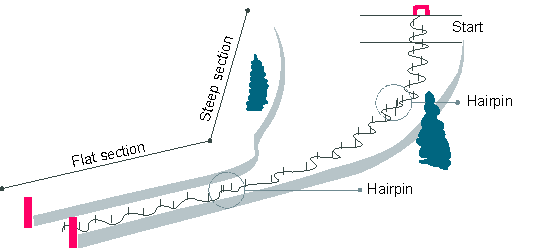
\includegraphics[width=1\linewidth]{figure/figure_introduction_course.pdf}
    \caption{Illustration of different section in a slalom race}
    \label{fig: flatcourse}
\end{figure}

\section{What can skiers do to improve their performance in flat sections in slalom?}
The next question is how skiers can increase their speed on flat sections in slalom. In this sport, performance boils down to how effectively athletes can utilize the mechanical energy available to them \cite{supej_differential_2008, supej_how_2010}. Therefore, this section first outlines the fundamental mechanical energy principles of skiing. Based on these principles and quantitative evidence from field research on elite skiers, I will propose four strategies to potentially enhance skier performance on flat terrain in slalom, which we wanted to study in this doctoal project.  

\subsection{Energy mechanics of alpine skiing}\label{introduction: energymechanics}
When skiers take the ski lift to the top, they  accumulate gravitational potential energy. This acquired potential energy is the skier's main engine \cite{supej_differential_2008, supej_mechanical_2011} and enables them to do work such as making the ski penetrate the snow to make it turn. The amount of potential energy available to the skier for performing such work at the top of a slalom course can be derived from the following equation:
\[U=mgh\]
Here, $U$ represents the gravitational potential energy (measured in joules), $m$ represents the mass of the skier (measured in kilograms), g represents the gravitational acceleration (approximately $m/s^2$) acting on the skier, and $h$ represents the height (measured in meters). When the skier descends the slalom course, the amount of work done by gravity can be derived by finding the gravitational potential energy for the initial position $U_1$ (e.g., at the top of the slalom course) and the gravitational potential energy for the final position $U_2$ (e.g., at the end of the first turn); then, the negative change in potential energy can be calculated: 
\[W=-U_2 + U_1\]
\[W= -\Delta U \]
This quantity represents the work of gravity on the skiers as they descend from the top to the lower position of the slalom course. According to the law of conservation of mechanical energy, all this work must be converted to kinetic energy when gravity is the sole force acting on the skier. The skiers' kinetic energy can be represented by the following equation:
\[ K = \frac{1}{2} m v^2 \]
where $K$ is the kinetic energy, $m$ is the mass of the skier, and $v$ is the velocity of the skier. Consequently, the sum of the potential and kinetic energy  (denoted as $E$ for mechanical energy) remains constant during a descent, as expressed by the following equation:
\[ E = U + K \]
During descents, however, skiers are exposed to two dissipative forces that oppose motion and can result in some loss of energy transfer to kinetic energy. For skiers, these two dissipative forces are air drag and snow friction (collectively denoted as $D$)\cite{supej_differential_2008}. Therefore, the total mechanical energy during a descent equals the sum of the kinetic energy and the dissipating forces (equation below), and is conceptually illustrated in Fig. \ref{fig:energy}.
\[ U = K + D\]
Consequently, in terms of the mechanical energy principle, a skier's goal during a descent should be to maintain high kinetic energy \cite{supej_differential_2008, supej_mechanical_2011, supej_how_2010}. One conventional strategy that most skilled skiers' employ to achieve this goal include carving instead of skidding \cite{supej_differential_2008, supej_relations_2006, reid_kinematic_2010, reid_turn_2009}. Are there solutions that can effectively improve performance on this section beyond the usual strategy? 

\begin{figure}[H]
    \centering
    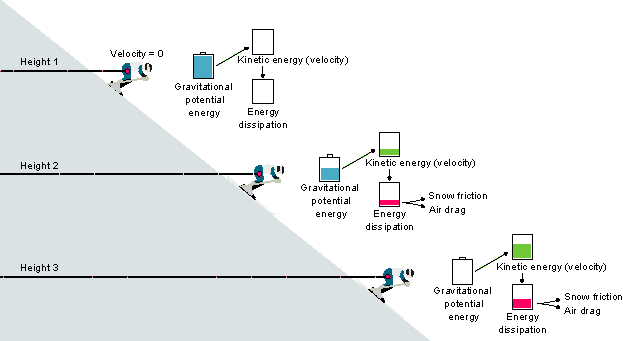
\includegraphics[width=1\linewidth]{figure/figure_introduction_mechenergy3.pdf}
    \caption{Illustration of mechanical energy in alpine skiing}
    \label{fig: energy}
\end{figure}



\subsection{Strategies to improve race times in flats in slalom}\label{introduction: strategies}
If most skilled skiers can execute clean, carved turns, what else can they do to achieve better performance on flats in slalom? Here, I outline four strategies that can potentially achieve this goal, all directed at improving energy mechanics management.  Fig. \ref{fig: strategies} illustrates these four strategies.  

The first strategy skiers could potentially use to maintain high kinetic energy during a turn and therefore improve their race times on flat sections in slalom is the 'stand against' technique. This strategien er nokså utbredt blant trenere i skimiljøet, og går ut på at skiers maintain a stable stance and actively resist being compressed toward their bindings by centrifugal force during a turn (from the skier's frame of reference). According to Lind and Sander's theoretical model on 'pumping to increase velocity' \cite{lind_physics_2004}, this active force resistance could minimize skiers' kinetic energy loss during a slalom turn by keeping the moment of inertia about the axis of rotation fixed instead of increasing it, as would occur if the skier collapsed during the turn. In their model, the rotational kinetic energy of a ski turn can be represented by the following equation: 
\[ T = \frac{L^2}{2I} \]
Here, $T$ represents the kinetic energy of rotation, and $L$ represents the angular momentum (that is, angular velocity ($\omega$) multiplied by the moment of inertia about the axis of rotation ($I = mr^2$)). Lind and Sanders considered a rider traveling on a cart on a friction-free rail with a curved turn and no torque to act on the system. In this situation, if the rider were to collapse toward the cart due to the centrifugal force, the moment of inertia would increase by lengthening the radius about the axis of rotation. Consequently, some rotational kinetic energy is lost if the skier fails to resist the centripetal force. Stand against might therefore be an effective strategy to ski faster on flats in slalom.  

A second and perhaps better strategy skiers can employ to maintain high kinetic energy during a turn is to 'rock skis forward'. By shifting their vertical position forward and backward, skiers regulate the ski’s total pressure distribution exerted against the snow\cite{lemaster_skiers_1999, lemaster_ultimate_2010, howe_new_2001}. This regulation not only helps skiers maintain balance but also affects the ski's turning behavior. For example, when skiers edge their skis, moving the center of mass toward the tip of the ski increases the pressure distribution on the ski's forebody, enabling it to turn more sharply. Conversely, if skiers edge their skis but shift their center of mass backward to the ski's tail, they decrease the pressure at the ski's forebody and consequently make the turn more gradual \cite{lemaster_skiers_1999, lemaster_ultimate_2010}. In ski racing, skiers generally aim to turn more sharply in the beginning and during the turn and should therefore shift their center of mass to distribute the pressure to the ski's forebody to make it engage with the snow. However, after gate passage, skiers generally aim to stop turning and should therefore shift their center of mass backward by rocking the skis forward. By rocking the skis forward after gate passage, skiers could in principle counteract the unnecessary loss of kinetic energy caused by the skis penetrating and digging unnecessarily into the snow in the exit of the turn. In support of this, previous research has found a strong linear relationship between the skier's forward position and energy dissipation \cite{reid_turn_2009, reid_kinematic_2010}. Additionally, faster skiers have shown to rock their skis more forward and pressure the back part of the ski for considerably longer during a turn compared to slower skiers\cite{reid_kinematic_2010, tjorhom_beskrivelse_2007}. Consequently, rocking skis forward could be an even better strategy than the stand against strategy for improving race times on flat terrain in slalom. 

The third strategy that can potentially make skiers faster on flat slopes in slalom is to 'extend,' also referred to as 'pumping' to increase velocity \cite{lind_physics_2004}. This strategy involves skiers moving their center of mass closer to the axis of rotation of a turn from a laterally inclined position by extending their legs. When the skiers extend this way, they can increase their kinetic rotational energy under certain situations. According to Lind and Sanders \cite{lind_physics_2004} model, the skier achieves this effect by shortening the radius of the axis about which they rotate, which will reduce the moment of inertia and consequently increase the rotational kinetic energy of the system under the assumption that angular momentum is conserved. In their model, the gain in rotational kinetic energy from this motion is proportional to the amount of work the skier does against the centrifugal force (from the skier's frame of reference); therefore, a larger extension movement will accomplish a greater increase in rotational kinetic energy. Scientists have previously assumed that the contribution of pumping to increase the velocity through a turn is minimal and an negotiable mechanism to leverage to improve skiers' race times\cite{supej_differential_2008}. Critics are directed that Lind and Sander's model neglects friction and that it only should work with low speeds \cite{supej_differential_2008, supej_how_2010}. Nevertheless, several studies has been observed that skilled alpine skiers gain additional kinetic energy at the exit of the turn—an increase that cannot be accounted for solely by their available potential energy at that moment\cite{reid_kinematic_2010, supej_how_2010, supej_differential_2008}. Moreover, in an experiment we conducted in 2012, elite skiers had better race times on a flat slalom section when they skied the course with the pumping technique than when they skied the section straight down, despite taking a significant longer trajectory in skiing the course. Therefore, "extend" could be a very important strategy.  

The final strategy is to "extend with rock skis forward", which combines "extend" and "rock skis forward". In a simulation study of skiers pumping on a an undulating terrain, this was the the best performing strategy \cite{mote_accelerations_1983}, and it has been suggested that this could be the best strategy to perform in slalom turns in certain situations \cite{reid_kinematic_2010}. We therefore considered this strategy as the theoretical best strategy. 

Although mechanical theory and quantitative evidence suggest that 'extend with rock skis forward' is an effective strategy on flat terrain in slalom, no or little experimental data on this topic exist. Et viktig spørsmål med doktorgraden var derfor å finne ut hvilke strategier gode skikjørere presterer best med på flater. D


Another important goal was to understand the impact of a training intervention focused on the pumping (or extend) strategy exerted on the kinematics of skiers. If skiers can pump themselves to higher velocities, it is crucial to investigate the kinematic changes involved. This understanding will help us better grasp what actually occurs when skiers pump. Therefore, another question was: what happens to a skier's kinematics when they learn to pump?


\begin{figure}[H]
    \centering
    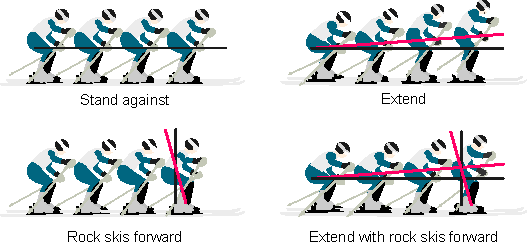
\includegraphics[width=1\linewidth]{figure/figure_introduction_strategies.pdf}
    \caption{Illustration of the strategies to improve reace times in flats in slalom}
    \label{fig: strategies}
\end{figure}



\section{What is the best way to teach these skills?}
The next question is whether insights from cognitive science can help coaches create more effective training. To ensure effective training, coaches generally have two main strategies for creating optimal learning situations at their disposal: designing learning problems for athletes and using effective teaching signals for instruction and feedback. In alpine skiing, skiers constantly face new slalom courses in races, requiring them to adapt their strategies and techniques. Therefore, their training should cover a wide variety of course scenarios to best prepare them to handle these diverse demands effectively. Given that coaches address this breadth of variation, should they also increase the frequency at which they expose their skiers to new learning problems? This is one of the questions we aim to test in this doctoral study. Another question is whether coaches can improve their use of instruction and feedback by selecting the most effective teaching signals.


\subsection{Can coaches improve skill learning by increasing the frequency at which they expose skiers to new learning problems?}
One learning effect that supports increasing the frequency at which coaches or teachers expose skiers to new learning problems is the contextual interference effect \cite{lee_contextual_2012, shea_contextual_1979, magill_review_1990}. This teaching strategy involves training learning problems (in our case courses) in a nonrepetitive sequence (that is, interleaved order), such as practicing learning problems A, B, and C in the order of BCA, ACB, or ABC, rather than a practice structure where problems are repeated in blocks (that is, blocked practice), such as AAA, BBB, or CCC. This nonsystematic training structure has been shown to be an effective teaching strategy for improving skill retention and transfer in various simple learning tasks \cite{tsutsui_contextual_1998, simon_metacognition_2001, shea_context_1983, shea_contextual_1979, tsay_signatures_2023}.

Two main explanations have been proposed to account for the contextual interference effect: the elaboration hypothesis \cite{shea_contextual_1979, shea_context_1983} and the reconstruction/forgetting hypothesis \cite{lee_can_1985, lee_locus_1983}. The elaboration hypothesis proposes that interleaved practices prompt individuals to process information more eloborately during acquisition, which enriches their understanding and problem solving techniques. This increased elaboration process enhances retention, which is not fully realized when practicing learning problems in a blocked order \cite{shea_contextual_1979, shea_context_1983}. In contrast, the reconstruction/forgetting hypothesis posits that increased problem switching provides more opportunities to forget task-relevant information held in working memory. This forgetting of task-relevant information forces the learner to reconstruct the action plan for every trial the learner revists the task. The repetitive process of abandoning and reconstructing action plans during interleaved practice contributes to better memory formation and thus increased retention \cite{lee_can_1985, lee_locus_1983}.

The contextual interference effect has not always succeeded in transferring to the learning of real-world skills, however \cite{wulf_principles_2002, brady_theoretical_1998, barreiros_contextual_2007, AMMAR2023100537, guadagnoli_challenge_2004}. This discrepancy can be understood through the challenge-point framework \cite{guadagnoli_challenge_2004} and recent extensions of it \cite{hodges_extended_2022}, where the effect of contextual interference is moderated by both the difficulty of the task and the skill level of the performer. In this framework, easy tasks can benefit from contextual interference to make the task more challenging, whereas difficult tasks are already challenging enough to serve as adequate learning stimuli on their own and are best learned without contextual interference initially. As the learner becomes more skilled, the learning process may benefit from increased contextual interference to improve the level of difficulty. In align with this prediction, studies have shown that beginners who learn skills when practice increases from blocked to interleaved practice learn better than those who use blocked or interleaved practice alone \cite{porter_systematically_2010, saemi_practicing_2012}. 

One prediction derived from the challenge point framework is that skilled athletes can benefit from interleaved practice to make training more challenging and therefore better. Consistent with this notion, \cite{hall_contextual_1994} found that skilled baseball players who practiced batting achieved better retention through interleaved practice than through blocked practice. In contrast, \cite{buszard_quantifying_2017} found no statistically significant differences in retention between tennis players learning to serve through interleaved practice and those using blocked practice. Instead, these researchers found evidence for improved transfer to new situations. Thus, it is not entirely clear whether contextual interference can be generalized to skilled performers. One idea is that contextual interference is more beneficial in open sports, where performers must constantly switch between different strategies to solve tasks, potentially making it important for alpine skiers \cite{farrow_chapter_2017, buszard_quantifying_2017}. An important aim of this study is to investigate whether the contextual interference effect can be used to improve the training of skilled performers. 

\subsection{Can coaches improve their instruction and feedback using reinforcement learning?}
Den andre treningsstrategien trenere kan bruke for å skape gode læringsbetingelser er gjennom gjennom teaching signalet de bruker for instruksjon og tilbakemeldinger. Although we exercise caution in generalizing and asserting that all coaches teach in a specific way, er det vanlig formen for teaching signal trenere bruker er instruksjonsbasert teaching \cite{williams_practice_2005, williams_effective_2023, hodges_modelling_2002}. In this approach, they offer performers a correct solution followed by corrective feedback. For instance, a ski coach may encourage the skier to take a shorter line around the gate and then further encourage the learner to shorten the line after a few trials. This teaching strategy can be likened to supervised learning in motor learning, where the difference between the desired strategy and the performer's movement outcome represents a teaching signal for skill improvement  \cite{jordan_forward_1992, wolpert_motor_2010, doya_complementary_2000}. Through practice, this teaching signal can bring the performer closer to executing what is assumed to be the correct choice. But is this teaching strategy truly the most effective approach for enabling learners to select and employ effective strategies? 

Supervised learning offers a promising approach for assisting learners in making informed strategy choices, yet it may also lead learners away from discovering the optimal strategy. First, the coach's advice may not be the optimal solution, as the strategy that coaches believes to be optimal does not always align with reality, even for the best-trained eye \cite{supej_impact_2019, cochrum_visual_2021}. Consequently, learners might be hindered to learn the best strategy when coaches opt for suboptimal strategies \cite{gray_plateaus_2017}. Worse, these learned suboptimal strategies might turn into habits that can be difficult to break \cite{popp_effect_2020}. Second, learners trained through supervised learning might also be constrained to adopting a single ('universal') strategy for all situations rather than acquiring a repertoire of strategies and discerning the most effective strategies for each specific scenario. Finally, it remains uncertain whether the prescriptive approach is the most effective teaching strategy for enabling performers to achieve long-lasting learning effects \cite{wulf_instructions_1997, hodges_role_1999, williams_practice_2005,williams_effective_2023}. 

Another, yet much less frequently adopted, teaching strategy to help learners learn to make good choices is through reinforcement learning \cite{sutton_reinforcement_2018}. The cornerstone of this approach is that the learner learns from evaluations instead of instruction, which occurs by using successes and failures of outcomes as teaching signals. That is, the performer learns the value of different strategies which allows them to finally pick the best solution, rather than being told the putatively correct solution to the problem. Specifically, these values are learned by comparing a given choice's outcomes with the choice's currently expected outcome. Outcomes that exceed or fall short of expectations result in errors in reward prediction, signaling that the learner must update their predictions to better anticipate future rewards following that action \cite{rescorla_theory_1972}. These reward prediction errors are then incorporated to form a new and better estimate of expected reward by updating expectations through a weighted running average. The computations underlying this form of value-learning of choices have been tremendously powerful in explaining human and animal learning \cite{waelti_dopamine_2001, schultz_neural_1997, pessiglione_dopamine-dependent_2006,lee_neural_2012, law_reinforcement_2009, tobler_human_2006} as well as training AI to perform complex tasks such as computer games starting from pixel inputs, only\cite{mnih_human-level_2015}. In addition, reinforcement learning has been shown to improve motor skill learning on simple tasks performed in the laboratory \cite{lior_shmuelof_overcoming_2012, abe_reward_2011, truong_error-based_2023, hasson_reinforcement_2015}. Based on this evidence, we ask whether reinforcement learning offers a better alternative for training learners to make better decisions about strategies than traditional supervised learning with a coach. 



\chapter{Aims}
The aim of this doctoral project was twofold. On the one hand, the project aimed to develop a better understanding of how to achieve better race times on flats in slalom and strategies to support this goal. In addition, the project aimed to understand the kinematic signatures of the "extend" (pumping) strategy by examining the kinematic changes after a training intervention on this strategy. On the other hand, this doctoral thesis aims to test whether learning theories from cognitive science can improve skill learning in sports through better problem-solving tasks and more effective teaching signals. The two overarching goals of this doctoral thesis are mutually important and have developed in parallel. Based on these goals, I have identified four research questions that the thesis aims to address:

\begin{itemize}
    \item Which strategies do skilled skiers perform best with on flat sections? (Study 2; not published as paper) 
    \item What are the kinematic changes resulting from a prolonged training intervention on the pumping strategy (or extend strategy)? (Study 1; Paper 2)
    \item How should coaches best distribute problem-solving tasks among skilled skiers? (Study 1; Paper 1)
    \item Which teaching signal is most effective for helping skiers learn to select effective strategies for skiing fast on flat sections?  (Study 2; Paper 3)
\end{itemize}












\chapter{Method}
\newcommand{\RNum}[1]{\uppercase\expandafter{\romannumeral #1\relax}}

\section{Study overview}
Studie \RNum{1} var å teste om kontekstuell interference kan bidra til å forbedre oppgavene utøverne blir satt til å løse. 

Studie \RNum{2} var å teste om reinforcement learning er en bedre læringsstrategi for å hjelpe utøvere til å ta gode strategivalg sammenlignet med tradisjonell coaching instruksjon (supervised learning). For å teste dette designet vi en læringsintervensjon som gikk over tre dager. I læringsintervensjonen brukte vi et between-subjects design og multi-armed bandit.  Studie \RNum{2} besvarte hvilke av disse strategiene som utøverne presterte best med. 


\begin{figure}[H]
\centering
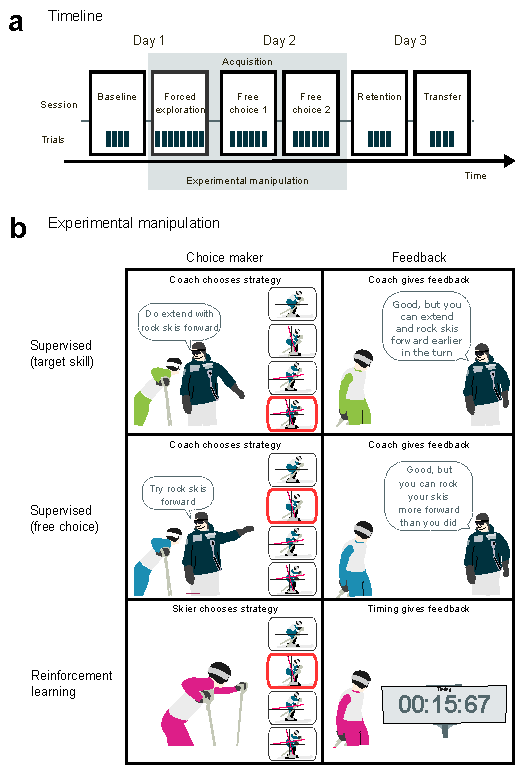
\includegraphics{figure_method_experiment.pdf}
\caption{Acceleration in the local positioning system section.\textbf{a.} Estimated acceleration during baseline and retention for the local positioning section. \textbf{b}. Expected mean difference between baseline and retention in the local positioning section.\textbf{c.} Estimated total gate-to-gate acceleration during baseline and retention in the local positioning section. \textbf{d}. Expected mean difference between baseline and retention in the local positioning section. The black lines denote the expected mean or differences in mean, with the shaded area representing their 95\% credible interval (CI). Each gray point or line represents one run trial by a skier}\label{fig: acc}
\end{figure}


\section{Setup}
All studies were conducted in the indoor ski hall, SNØ, located in Oslo, Norway (\url{https://snooslo.no/}). In this ski hall, we used the upper part of the race hill, which is a long flat section with two small rollers. The snow of this flat section was watered before testing each group of skiers to ensure uniform and fair conditions for all skiers. 

In study \RNum{1}, we set up three slalom courses to test the contextual interference effect. These courses required skiers to execute pumping movements with different timings and amplitudes for effective performance. All three courses had a vertical gate distance of 10 meters due to space constraints, forcing parallel setup. However, the courses had varying offsets: 1.2 meters for Course A, 1.7 meters for Course B, and 2.2 meters for Course C. These specific gate offsets were chosen to create diverse pumping demands without making it impossible to pump. Fig. 

In study 2, we set up two slalom courses to test. The main slalom course was used in all sessions except the transfer test and featured a 10-meter distance and a 1.9-meter offset. The transfer test assessed skiers' ability to transfer learning to a more realistic alpine race course. This test course included a progression in gate offset: five gates at 2.2 meters, seven gates at 1.7 meters, and seven gates at 1.2 meters. 

In both studies, we used stubbies (short gates) instead of long gates to minimize energy dissipation upon hitting the gate\cite{minetti_biomechanics_2018}. Using stubbies allowed skiers to focus better on skill execution of the strategy without the distraction of clearing the gate, which could hinder learning. In addition, this approach minimized hole creation that occurs when a long gate is forcefully slammed into the ground. 

We adopted the same standardized start procedure in both studies. The involved setting the start gate 20 meters before the first gate. Here, skiers were instructed to place their toe bindings behind the starting gate. Upon receiving the clearance signal, skiers were to place their skis parallel, lift the poles from the ground, and glide out of the start gate without using poling or skating to generate propulsion. Timing was recorded using a wireless photocell timing system (HC Timing wiNode and wiTimer; Oslo, Norway), starting when the skier crossed the first photocell pair situated 10 meters below the starting gate. (See https://osf.io/9numq for a supplementary video illustrating the starting procedure and setup).


\subsection{Participants}
Conducting studies on skilled alpine skiers presents several recruitment challenges. First, the population of skilled alpine skiers is relatively small and geographically dispersed across the country, which limits the number of participants available for testing. Additionally, these skiers must be willing to participate in the project. For coaches and skiers at this level to show this willingness, they must be convinced that the intervention will benefit the skiers' development, as it typically replaces the skiers' regular training due to their already high training volumes. Another limitation is the narrow time window for testing, typically in the spring and summer. This period is also popular for many ski teams to train indoors, leading to high demand for training lanes. Therefore, effective collaboration with the ski hall is crucial to gain permission to conduct research despite the high demand and to ensure the necessary support for the study. However, the ski hall can accommodate such studies only during a limited time of the year, further restricting the intervention period. These combined factors make it difficult to recruit a large number of participants.

Due to these resource constraints, our sample size approach in both studies was to recruit as many skiers as possible during the available testing window. To ensure that the skiers could handle the specific icy snow conditions prepared in the ski hall, we recruited skiers aged 15 years or older. Although some younger skiers participated in Study 1, they possessed the necessary skill level for the conditions. Beyond these criteria, we deliberately opted to recruit skiers with diverse skill levels to enhance the generalizability of our findings, despite not explicitly stating this in Study 1. In Study 1, we were uncertain about the expected effect sizes and our smallest effect size of interest, leaving our smallest effect size of interest unspecified. However, we learned much from this study. In Study 2, we set our smallest effect size of interest at a 0.3 second difference between groups. This benchmark was based on our knowledge of alpine skiing and discussions with coaches. However, it was intended for a 50-meter longer course and more training sessions than we ultimately used due to practical considerations. For Study 2, we set the minimum sample size to 80 skiers, which we deemed appropriate for this context. Prior to data collection, we conducted power simulations for sample sizes of 80, 100, and 120 skiers. These simulations revealed powers of 0.60, 0.75, and 0.80, respectively, for the smallest effect size of interest (0.3 seconds difference between groups) (\url{https://osf.io/c4t28}). 


\section{Design and procedure}

\subsection{Study 1}
In Study 1, we employed a between-subjects design and allocated skiers to either a blocked or interleaved learning group. The experiment began with a baseline test consisting of nine trials (three trials on each of courses A, B, and C), where skiers skied as quickly as possible without receiving time feedback. The trials in these courses were distributed randomly to each skier under the condition that the skier did not perform two consecutive runs on the same course. In addition, the skiers performed a straight gliding task on a dedicated lane before, midway (randomly assigned), and after the nine trials.

After the baseline test, we used a randomized-blocked design to allocate skiers into either the blocked or interleaved learning group based on their baseline test times. Specifically, we extracted each skier's best run from the baseline on each course and divided it by the average of the straight gliding runs from the baseline. Skiers were then ranked from fastest to slowest and paired in ascending order, and each consecutive pair was randomly assigned to either the interleaved or blocked group.

Immediately after the baseline test on day one, skiers attended a workshop where we explained the mechanical principles of the pumping technique and presented quantitative evidence supporting this strategy. Skiers then completed three training sessions over three days, with each session including 15 runs: 12 runs on the three courses and three straight-gliding runs. The interleaved group skied all three courses each day in a randomized interleaved order, ensuring no more than two consecutive runs on the same course. The blocked group performed all their runs on one course (A, B, or C) per day, with the course order counterbalanced across participants. 

Three days (72 hours) after the last training session, the skiers returned for a retention test, consisting of 12 runs (three runs on each of the three slalom courses and three straight-gliding runs). The order of the runs in the courses was scheduled in a semirandom order, with the condition that no more than two consecutive runs could be performed in the same course. As in the baseline test, the skiers performed a straight gliding task on a dedicated lane before, midway (randomly assigned), and after the nine trials. The skiers were instructed to ski as fast as possible but did not receive any performance feedback during the posttest. This design allowed us to compare the effects of blocked versus interleaved practices on the learning and performance of the pumping strategy. 


 \subsection{Study 2}
In study 2, brukte vi et between-subjects design og framet oppgaven om å velge gode strategier som et multi-armed bandit problem \cite{sutton_reinforcement_2018} (see methodeseksjonen i paper 3 for en beskrivelse av dette problemet). I denne studien var valgmulighetene (eller bandits) som utøverne måtte lære handlingsverdien og velge for å kjøre raskest mulig på ski de fire tekniske strategien vi har utbrodert i seksjon \ref{introduction: strategies}. 

Læringseksperimentet begynte med en baseline som bestod av fire runder i slalåmløypen (main course in fig), pluss en straightgliding runde der utøverne kjørte ned løypeseksjonen i en egen dedikert bane for dette. Før utøverne gjennomførte disse fire rundene og straight glidingen gjennomførte de to oppvarmingsrunde: en gjennomført som frikjøring og som gjennomført som oppvarming i løypen, der de fikk instruksjoner og tilbakemelding på utførelsen av startprosedyren. 

Etter dette delte allokerte vi utøverne i tre læringsgrupper











































\chapter{Results and discussion}

\subsection{How do skilled performers perform better on flat section in slalom?}


\subsubsection{Which strategies are best to perform well on flats?}
We began by studying which technical strategies enable skilled alpine skiers to descend a flat slalom course as quickly as possible. The strategies we examined in study 3 were "stand against," "rock skis forward," "extend," and "extend with rock skis forward." We began testing after a familiarizing session where we introduced skiers to the strategies and allowed them to practice until they understood and mastered the techniques. Once understood, the skiers performed a total of eight trials (two on each strategy) that were randomly assigned to each skier under the condition that the first and last four trials included all four strategies. Therefore, we could use the data to estimate which technical strategies enable skilled alpine skiers to descend a flat slalom course as quickly as possible.

We employed a Bayesian modeling approach (model 1) to estimate the differences between the strategies. The analysis revealed that skiers on average achieved their best descent times using the 'extend with rock skis forward' strategy (16.66, 95\% credible interval (CI) = 16.54, 16.77). The second best strategy for skiers was to step down to solely "extend," which was only 0.02 sec. (95\% CI = -0.02, 0.06) slower than the "extend with rock skis forward" strategy. However, when skiers switched from the "extend" strategy to the "rock ski forward" strategy, the expected time loss was 0.21 sec. (95\% CI = 0.16, 0.25). Finally, if the skiers switched from the "rock skis forward" strategy to the "stand against" strategy, the expected time loss was 0.2 sec. (95\% CI = 0.15, 0.25). Therefore, the strategies the skiers used made a great difference in race time.

The results show that just skiing cleanly and resisting centripetal forces during a turn does not suffice to achieve fast race times on flat terrain in slaloms. Instead, the active movements of the skiers were crucial for achieving good race times on flats. "Rock skis forward" resulted in significant improvements in race times compared to 'stand against'. This finding aligns well with prior findings in slalom skiing, showing a strong correlation between fore and aft movements and energy dissipation, such that more fore movements are associated with greater energy dissipation \cite{reid_turn_2009, reid_kinematic_2010}. Furthermore, studies have shown that faster skiers have a greater range of fore/aft motion and spend a larger portion of the turn skiing with their weight shifted back after gate passage than slower skiers \cite{tjorhom_beskrivelse_2007, reid_kinematic_2010}. Our results extend these findings and provide experimental evidence that "rock skis forward" can be an effective strategy for improving race times on flat terrain in slalom.

The 'rock skis forward' strategy resulted in much slower times than did the 'extend' strategy, however. Predictions from the Lind and Sanders model \cite{lind_physics_2013} indicate that extending the center of mass closer to the axis of rotation during a turn from a laterally inclined position should significantly improve the race time. Without motion capture data, we cannot assess the extent to which skiers extended and the resulting increase in kinetic energy. Nonetheless, the results suggest that skiers' extension movements play a crucial role in slalom performance, contrary to previous claims \cite{supej_differential_2008}.

Finally, we found that "extend with rock skis forward" on average was the best strategy. This finding aligns with previous simulations suggesting that this strategy is most effective when skiers pump over rollers \cite{mote_accelerations_1983} and that it can be transferred to skiers executing a turn \cite{reid_kinematic_2010}. However, it is important to emphasize that "extend with rock skis forward" only was marginally better than the "stretching" strategy alone. One reason for the limited improvement achieved by adding "rock skis forward" to the "extend" strategy might be that rocking the skis forward during the turn compromised how much the skier could extend toward the turn's axis of rotation. For instance, extensive extension could be challenging if the skier's center of mass was located at the tail of the skis. This issue should be further investigated in future analyses.

One limitation of these timing analyses is that we do not have precise knowledge of how much the skiers moved when executing the strategies or how these strategies affected the mechanical energy during a turn. Therefore, we cannot comment on the skiers' actual execution or the energy mechanics behind each strategy. Future studies should incorporate motion capture to address this gap in understanding.



\begin{figure}[H]
\centering
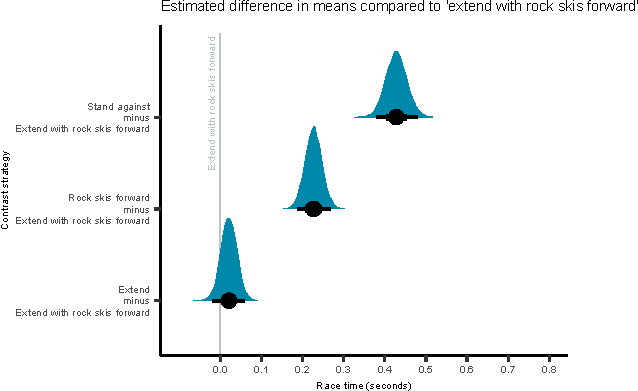
\includegraphics{figure_results_Q1_strategies.pdf}
\caption{Estimated differences in means compared to 'extend with rock skis forward'. The circle represents the point estimates whereas the shaded distribution represents the posterior distribution fitted from the model}
\label{fig:q1_strategieseffect}
\end{figure}



We found that the skiers improved their race times in both the intermediate split and the local positioning sections, which inspired us to continue studying the kinematic changes among skiers in the local positioning section. If the improvement in the skiers' race times can be attributed to the pumping mechanism, we would expect skiers to increase their velocity around or immediately after gate passage, at the time when the extension movement occurs.  Figure \ref{fig: velocity}a shows the velocity profiles for the local positioning system section during baseline and retention. We first describe the global velocity trend at baseline and then the contrast between baseline and retention.

Before the intervention (baseline), the skiers' velocity nearly declined for every gate in the local positioning sequence compared to their velocity during straight gliding. With the exception of a slight velocity increase of 0.05 m/s (95\% CI [-0.08, 0.17]) from gate 1 to gate 2, the velocities decreased on average by -0.06 m/s (95\% CI [-0.19, 0.07]) from gate 2 to gate 3 and by -0.12 m/s (95\% CI [-0.25, 0]) from gate 3 to gate 4 compared to straight gliding times. We focused only on comparisons at the gates because the gates mark a fixed reference point. 

After the training intervention, skiers increased their entry velocity into the local positioning section (gate 1) by an average of 0.24 m/s (95\% CI [0.19, 0.29]) compared to the baseline velocity. However, the skiers also tended to increase their velocity throughout the section. Specifically, the skiers increased their velocity on average by 0.07 m/s (95\% CI [0.01, 0.12]) from gate 1 to gate 2, followed by a slight decrease of -0.02 m/s (95\% CI [-0.05, 0.02]) from gate 2 to gate 3. Subsequently, the velocity of the skiers increased again by 0.1 m/s (95\% CI [0.06, 0.14]). Therefore, the velocity of the skiers increased almost incrementally from gate to gate. Besides, the velocity profiles appeared more wavy, as depicted in Fig. \ref{fig: velocity}b. In general, the pattern of these waveforms was that skiers increased their velocity after gate passage and continued to rise until the skier was between two gates. After that, the velocity decreased to the6 gate passage before it rose again. 

\begin{figure}[H]
\centering
\includegraphics{figurer/figure_velocity_3.pdf}
\caption{Velocity in the local positioning system section. \textbf{a.} Estimated velocity during baseline and retention for the local positioning section. \textbf{b}. Estimated differences (contrast) between baseline and retention for the local positioning section. The black lines denote the expected mean or differences in mean, with the shaded area representing their 95\% credible interval (CI). Each gray point or line represents one run trial by a skier}\label{fig: velocity}
\end{figure}

\subsection{Acceleration}
We continued examining acceleration through the turn to analyze the velocity changes more closely. As shown in Fig. \ref{fig: acc}a, the acceleration exhibited fluctuating waves, with skiers increasing their acceleration up to about the switch between two turns that began just before or around the gate passage. After this switch, the skiers decelerated until just before the gate. 

During the baseline, we found that the skiers' acceleration decreased on average by -0.91 m/s$^2$ (95\% CI [-1.71, -0.05]) from gate 1 to gate 2, followed by an increase of 0.42 m/s$^2$ (95\% CI [-0.40, 1.31]) from gate 2 to gate 3 and then a marginal increase of 0.01 m/s$^2$ (95\% CI [-0.84, 0.79]) again from gate 3 to gate 4, compared to the acceleration during straight gliding.

Following the intervention, the skiers developed a significantly more wavy acceleration profile with higher peaks and lower troughs compared to the baseline. We performed a gate-to-gate analysis, which revealed that acceleration was lower at gate 1 by -0.53  m/s$^2$ (95\% CI [-0.66, -0.41]), at gate 2 by -0.19  m/s$^2$ (95\% CI [-0.26, -0.13]), at gate 3 by -0.48  m/s$^2$ (95\% CI [-0.54, -0.42]), and at gate 4 by -0.42  m/s$^2$  (95\% CI [-0.48, -0.36]) compared to the baseline. Fig. \ref{fig: acc}b shows the expected mean difference between baseline and retention. 

To better understand how the acceleration changed between baseline and retention in each turn, we computed the total acceleration from gate to gate through the local positioning sequence. From this model, we found that the estimated difference in total acceleration was 24.4 (95\% CI [-14.4, 63.1]) from slalom gate 1 to slalom gate 2, 1.65 (95\% CI [-37.6, 40.1]) between gate 2 and gate 2, 39.4 (95\% CI [0.59, 78.1]) from gate 3 to gate 4, and 107.0 (95\% CI [68.8, 146.0]) from gate 4 to the end of the sequence. Therefore, the skiers appears to have had a positive overall acceleration in most of the gates in the sequence. Fig. \ref{fig: acc}c and d show the total acceleration during each gate in the local positioning section.

\begin{figure}[H]
\centering
\includegraphics{figurer/figure_acc_2.pdf}
\caption{Acceleration in the local positioning system section.\textbf{a.} Estimated acceleration during baseline and retention for the local positioning section. \textbf{b}. Expected mean difference between baseline and retention in the local positioning section.\textbf{c.} Estimated total gate-to-gate acceleration during baseline and retention in the local positioning section. \textbf{d}. Expected mean difference between baseline and retention in the local positioning section. The black lines denote the expected mean or differences in mean, with the shaded area representing their 95\% credible interval (CI). Each gray point or line represents one run trial by a skier}\label{fig: acc}
\end{figure}

\subsection{Path length}
Finally, we analyzed the path length, which we expected not to undergo massive changes according to our measurements from the local positioning system. In the case of change, we would expect it to be shorter during retention than during baseline because skiers (theoretically) would ski a shorter path length as they extended toward the axis of rotation during the turn.

At baseline, we found that the total path length from gate 1 to gate 2 was 91.53 (95\% CI [83.86, 99.30]), 92.57 (95\% CI [84.75, 100.45]) from gate 2 to gate 3, and 87.30 (95\% CI [79.40, 95.32]) from gate 3 to gate 4, while it was 69.30 (95\% CI [61.35, 77.16]) from gate 4 to the end of the section. Notably, the reason for the lower estimate from gate 4 to the end is that this section was shorter than the other sections. Fig. \ref{fig: path}a shows the total path length during each gate in the local positioning section.

\begin{figure}[H]
\centering
\includegraphics{figurer/figure_path.pdf}
\caption{Total path length in the local positioning system section.\textbf{a.} Estimated total path length during baseline and retention for the local positioning section. \textbf{b}. Expected mean difference in total path length between baseline and retention in the local positioning section. The black lines denote the expected mean or differences in mean, with the shaded area representing their 95\% credible interval (CI). Each gray point or line represents one run trial by a skier}\label{fig: path}
\end{figure}

As expected, we found only marginal differences between baseline and retention in total path length. The expected mean difference was -2.73 (95\% CI [-13.8, 8.23]) from gate 1 to gate 2, -2.08 (95\% CI [-12.9, 8.99]) from gate 2 to gate 3, and -1.99 (95\% CI [-13.3, 9.18]) from gate 3 to gate 4, while it was -1.4 (95\% CI [-12.3, 9.62]) from gate 4 to the end of the section. Thus, there was considerable overlap in the expected differences in the mean difference in total path length. Fig. \ref{fig: path}b shows the expected mean difference in total path length during each gate in the local positioning section.

\section{Problem solving}
Our next question was whether coaches can improve skiers' training by using contextual interference to improve their problem-solving skills. In our study, skiers trained to pump on flat sections in slalom either in one course per day (blocked practice) or in different course 34s that were randomly assigned to each skier (interleaved practice). According to the typical results of the contextual interference effect \cite{simon_metacognition_2001, shea_context_1983, hall_contextual_1994, shea_contextual_1979}, we initially hypothesized that the blocked group would perform better during the training sessions (acquisition) than the interleaved practice group, as they had repeated opportunities to perform on the same course (thus experiencing less interference). På de første fire trialsene (trial block 1), fant we ingen statistisk signifikante forskjeller mellom interleaved og blocked practice. We 







Det kan være flere grunner til at kontektuell interferens effekten ikke fremkom i vår studie og som bryter med funn fra tidligere studier. Den mest åpenbare forklaringen var at utøverne i vår studie var gode utøvere og at de trente en langt mer kompleks ferdighet enn det som har blitt gjort i tidligere studier. En sammenlignbar studie med vår var \cite{buszard_quantifying_2017} som heller ikke fant effekt av kontektuell interferens på trening av tennisserver hos yngre utøvere. Disse forskerne rapporterte kun en effekt på øverføring til nye situasjon. 





Our next question was whether coaches can improve skiers' training by employing contextual interference to enhance their problem-solving skills. I vår studie trente utøverne på å pumpe på flater i slalåm enten i en løype per dag (blocked practice) eller i forskjellige løyper som var tilfeldig for hver skikjører (interleaved practice). Jamfør med på kontekstuell interferens effekten typiske resultater, var vår hypotese først at blocked gruppen skulle gjøre det bedre under innlæring enn interleaved practice som følge av at de får gjentakende muligheter til å prestere i samme løype (og dermed lite interferens). For å teste dette nummerte vi rundene fra 1 til 12 og batched de inn i trial blocks 1 (run 1-4), 2 (run 5-8) og (9-12) i henhold til tidligere kontekstuell interferens studier. Under den første av disse blockene fant vi ingen statistiske signifikante forskjeller mellom gruppene for verken løype A, B eller C. Vi fant at begge gruppene utviklet seg signikant fra trial block over disse trial blocksene. Vi fant derimot ingen statistisk signikant forskjell i forbedring hos de to gruppene. 

d\begin{figure}
    \centering
    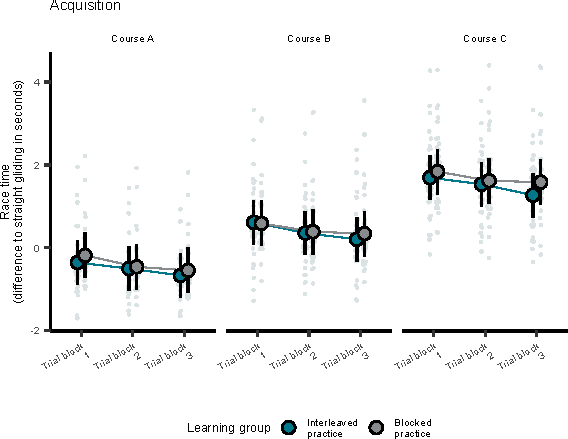
\includegraphics[width=1\linewidth]{figure/figure_results_ci_acquisition.pdf}
    \caption{Enter Caption}
    \label{fig:enter-label}
\end{figure}



\section{Methological considerations}


\chapter{Disussion}




\chapter{General discussion}














In recent decades, cognitive science has accentuated our understanding of the mechanisms that subserve skill learning, and sparked hope for more effective teaching strategies. However, most studies have leaned toward simple, laboratory-based tasks, raising concerns about their applicability to real-world learning in areas such as sports, education, or rehabilitation. Therefore, there is a pressing need for studies with greater ecological validity, where learning tasks are not trivial exercises but instead improve important life functions or skills that learners genuinely care about. The overarching goal of this doctoral thesis was to bridge this gap between simple tasks and real-world skill learning with skilled performers using alpine skiing as a domain to test these theories. To achieve this goal, this doctoral thesis used a crossdisciplinary research approach that combined mechanics and psychology. In this approach, mechanics was used to build knowledge about strategies that can help skilled skiers perform better on flats in slalom, while psychology offered knowledge of relevant learning theories that could improve learning in this learning context. Building on this approach, this doctoral project had two main subgoals: first, to identify effective strategies for skiing faster on flat slopes and to understand the kinematic signatures that make these strategies effective; second, to determine whether learning theoreis from cognitive science can improve skill learning for performers by creating more effective problem-solving methods and the use of effective teaching signals.

For det første fant vi at skiers i snitt kjørte raskest mest "extend with rock skis forward", som samstemte med våre forventninger basert på teorier og kvantitative observasjoner fra feltet. Det ser dermed ut til at denne strategien var en powerful strategi. Effekten av denne strategien var riktignok kun marginalt bedre enn "strekk" strategien som var en enklere strategi og som nesten ga full effekt alene. Basert på disse resultatenene vil vi anbefale utøvere å velge en av disse to strategiene for å forbedre prestasjoner på flater i slalom. Med disse resultater we expand earlier ski research and give experimental evidence about effective strategies to ski fast on flats in slalom. 

Vi fant også en treningsintervensjon på "extend" strategien etterlot seg en interessant kinematisk signatur på utøveres skikjøring. Etter intervensjonen fant vi at utøverne sin fartsprofil var betydelig mer bølgeformede, der skiers increased their speed after gate passage which continued to rise until they were approximately midway between two gates. After that, the speed decreased to the gate before it rose again. I tillegg fant vi en trend til at utøverne kjørte en lenger path length mellom gates, men til tross for at renntidene ble bedre. Den kinematiske signaturen minner dermed veldig om prediksjonene fra Lind and Sander's modell på pumping. I begrensning med disse dataene er at vi ikke vet hvilke bevegelser utøverne faktisk gjorde, og vi har dermed i mulighet for å teste prediksjonene fra modellen. Fremtidig forskning bør gjøre nærmere undersøkelser med motion capture for å oppnå denne nødvendige datakvalitaten.

Forflytter oss bort fra strategienes effekter og til testing læringsteoriene, fant vi ingen statistisk signifikant learning effekt av contextual interference to increase the frequency at which skiers are exposed to new learning problems. This finding aligns with previous research that has not found a contextual interference effect in real-world tasks or more complex activities \cite{brady_theoretical_1998, barreiros_contextual_2007, wulf_principles_2002}. Basert på resultatene fra denne og disse tidligere studiene er det ikke verdt effort å sette mange forskjellige slalomløyper iallefall når det kommer til prestasjon. Vi skal likevel ikke utelukke at å exponere utøvere for rapid bytter av løyper kan exert influence på andre kognitive mekanismer som motivasjon og som vi ikke har målt i denne studien. Det kan også være at gevinsten av å bytte løyper ofte er at man skal unngå habits, som at utøvere finner en løsning og blir insensitiv til å endre løsning til andre situasjoner. I så fall kan det muligens være nok å bytte løyper tilstrekkelig ofte slik at man unngår disse habitene. For å bedre forstå dette er det viktig med et annet eksperimentelt design. En måte å gjøre dette på er å trene hårnåler der en læringsgruppe kun trener en hårnål, mens en annen gruppe trener flere hårnåler. 















Our data indicate that the intervention increased the speed and path length in certain gate sections. How does this align with previous alpine research and mechanical theories on pumping? First, these and previous results suggest that the pumping ("extend") strategy might exert a real impact on skiers' speed and performance in flat sections, contrary to previous beliefs \cite{supej_differential_2008, supej_doba_2001}. The increased speed from turn to turn and the distinct change in the speed profile align well with expectations from a pumping mechanism to increase the speed from turn to turn. It therefore appears that skiers can pump themselves to higher speeds and that this is an important mechanism to leverage in align with Lind and Sander's model \cite{lind_physics_2004}. We also observed a trend where the path length increased slightly from gate to gate, although this varied significantly from turn to turn. Several factors could explain this increased path length, which we cannot quantify or separate using the local positioning system. One possibility is that pumping increases the path length because the extension movement exerts more force on the skis, causing them to bend and turn more. However, this could also result from measurement errors from the local positioning systems or differences in the course setting.

























og denne studien er den første som gir eksperimentell evidens for at utøvere 


men strategien var riktignok kun marginalt bedre enn å strekke alene. Det ser dermed ut til at å strekke i seg selv var en powerful strategi. Utøvere bør derfor bruke ekstend eller extend with rock skis forward når de kjører flater. Når imidlertid helningsvinkelen øker og det blir vanskeligere å bruke disse strategiene bør utøvere bytte strategi. Den utfordrende oppgaven er å finne ut når man kan bruke ekstend og når man skal bruke andre strategier. Dette er interessant å studere i videre forskning.

For det andre så vi at


Vi fant også at reinforcement learning var et effektivt teaching signal som kan brukes for å trene gode athletes. 















our research strategy was to develop knowledge about the skills and strategies that 


these skilled performers use to enhance their performance further and actively use this knowledge to create interventions for relevant skills to test these learning theories. This dissertation had two main objectives: first, to identify the most effective strategies for high-speed performance on flat surfaces and to understand why these strategies are effective; second, to determine whether cognitive science learning strategies can improve learning situations for performers through more effective problem-solving methods and the use of effective teaching signals. 






In recent decades, cognitive science has accentuated our understanding of the mechanisms that likely exert control of skill learning, og øynet håp om hvordan de kan utnyttes bedre for mer effektive læring. However, most of these studies have been performed with simple, laboratory-based tasks, raising concerns about their generalizability to real-world learning, such as sports, education, or rehabilitation. Therefore, there is a pressing need for studies with greater ecological validity, where the learning task not is a trivial exercise but may improve important life functions or skills that learners genuinely care about. Det overordnede målet med denne doktorgraden var derfor å bridge dette gapet mellom enkle oppgaver og komplekse real world skills med gode utøvere. Den valgte forskningtilnærmingen for å få til denne bridgingen var å bygge opp kunnskap om ferdigheter og strategier som disse gode utøverne kan bruke for å løfte prestasjonen videre, og deretter aktivt bruke denne kunnskapen til å lage intervensjoner på relevante ferdigheter for å teste disse læringsteoriene. Doktorgraden har således hatt to hovedmål: for det ene var det å finne ut hvilke strategier som er mest effektive for å kjøre raskt på flater og å forstå hvorfor disse strategiene er effektive. For det andre var det å forstå om disse læringsstrategiene fra kognitive vitenskap kan brukes til å forbedre læringssituasjoner hos utøvere gjennom mer effektive måter å lage læringsproblemer på og bruk av effektive teaching signals.

Det første spørsmålet som ble addressert i denne doktorgradenvar om 



Cognitive science has made great strides in understanding the mechanisms that likely exert control of skill learning and how they can be leveraged to improve learning and performance \cite{wolpert_principles_2011, makino_circuit_2016, spampinato_multiple_2021, krakauer_motor_2019, haith_model-based_2013, huang_rethinking_2011, shmuelof_are_2011, doya_complementary_2000}. 






\subsubsection{Quantifying performance in alpine skiing}
One of the key objectives of this doctoral project was to determine a reliable method for quantifying performance in alpine skiing over time, whether over days, weeks, or months. One of the greatest challenges in this respect, from a scientific perspective, is its lack of standardization; the time taken to ski a slalom course one day may not be comparable to that of another day  Consequently, quantifying performance in alpine skiing has been widely debated, with scientists arguing for measures such as energy mechanics \cite{supej_differential_2008, supej_how_2010, supej_mechanical_2011} , differences in mechanical energy divided by time, section times \cite{supej_relations_2006}, lateral skidding of skis \cite{kirby_development_2009}, and time loss per elevation difference and distance travelled per elevation difference \cite{federolf_quantifying_2012}. Throughout my doctoral research, I have chosen to express performance in terms of time, which is the conventional way to quantify performance in skiing and allowed me to operate on the same scale as skiers and coaches do. In my doctoral reseach, I have adopted two different time measures: in papers 1 and 2, I have expressed time as the difference from the time when the skier skied the section straight down (straight gliding), whereas, in paper 3, I used the raw time to quantify performance. Here, I aim to provide some methodological reflections on these approaches to help readers evaluate the results of the studies in this doctoral thesis and to assist other researchers in the field of alpine skiing. 

To begin this methodological consideration, I conducted a Bayesian multilevel growth model on all the skiers' times as they skied straight down the section for all sessions in paper 3. From this analysis, I found that the straight gliding times for all ski groups (A, B, C, and D) increased steadily from the first session (baseline) to the last session (transfer). Although I cannot rule out any explanation for why the straight gliding times of the ski groups increased uniformly, I am confident that differences in the length of the course section are not the main explanation. This is because we used a measuring tape during the course setting, and there was a tight cluster of boreholes at the finish line, with only a few centimeters of difference. I also do not believe that changes in the skiers' starting procedures or execution of straight gliding are the main reasons. This is because the skiers were diligent and interested in performing this task as well as possible. I believe the best explanation involves the snow conditions and how we prepared them. Specifically, when grooming snow with a machine, grooves are left in the snow that becomes hard if it is watered and allowed to freeze. These hard grooves are fast to ski on because only a small part of the ski is in contact with the snow surface. As skiers complete more runs and coaches slide through the course, these snow grooves wear away, creating a smooth, hard base without grooves. When skiers descend on this groom-free base, a larger part of the ski’s contact surface touches the snow, which increases ski–snow friction and slows the skiers down.

The question is, what consequences does this have for the results, and how can we address these challenges the best possible way? First, one challenge this creates is the need to exercise caution in interpreting 'true' learning from the estimated change in race times. From From Fig. \ref{fig:rlstudy_racetime} from Study \RNum{2}, we find that the skiers improved their race times significantly over the sessions despite the increased straight gliding times. Therefore, the 'true' improvement is likely better than estimated. A less conservative and perhaps better way to express skiers' 'true' learning is to use the difference in straight gliding times for each session to account for variations in the snow surface. This is the performance measure we used in Study\RNum{1}. However, although this measure may better capture skiers' learning, we do not know whether it underestimates or overestimates learning. Another problem is that straight gliding in itself is a random variable that introduces variation and could add noise to the measurement. In Study \RNum{2}, we had to move away from this measure because the straight gliding lane crossed many holes from the previous courses. Due to these challenges, it is difficult to determine the actual improvement of skiers. Scientists therefore face two choices: either use raw race times, which is likely a conservative method that underestimates the real improvement, or express time as the difference in straight gliding, which may better account for variations in the surface and therefore express progress more accurately. The cost of the latter approach is that it underestimates or overestimates performance and could increase noise. 

Another solution is to downplay the focus on change and determine whether the learning groups differ on the postmeasure if their performance is equal at baseline, corresponding to the logic of an ANCOVA. If we have a design where skiers have undeone tests simultaneously, we can estimate this group difference, indirectly avoiding the question of change. Therefore, we used ANCOVA and raw race data in Study \RNum{2}.

One potential way to improve estimates in future research is to test more levels within the ski groups. This would allow the groups to have varying effects of the treatment and achieve better estimates through partial pooling \cite{mcelreath_statistical_2018}. We attempted to run this model, but it did not converge due to having too few levels. It might have been better to divide the ski groups into smaller subgroups that were tested at different times. This approach could have provided more levels and potentially better estimates through partial pooling. However, it must be emphasized that conducting studies such as ours is very difficult and time-consuming. Another approach is to skid extensively to eliminate the grooms before testing. 


\begin{figure}
    \centering
    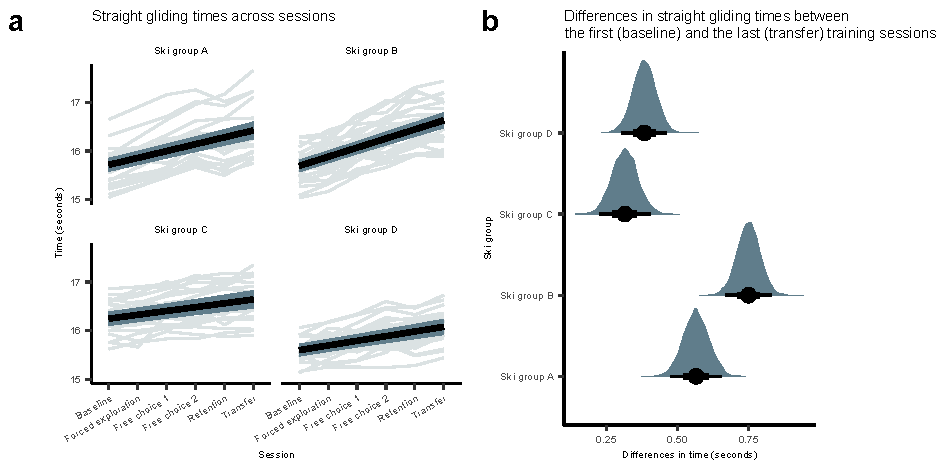
\includegraphics[width=1\linewidth]{figure/figure_methodological_straightgliding.pdf}
    \caption{Enter Caption}
    \label{fig:straightgliding}
\end{figure}

\chapter{Appendix}

\begin{table}[ht]
\centering
\caption{Race times: change per course for each treatment}\label{paper1: racetimechangepercourse}
\begin{tabular}{llrrrrrrl}
  \hline
Term & Estimate & SE & df & CI & t & p \\ 
  \hline
(Intercept) & 0.52 & 0.21 & 5.81 & -0.01-1.05 & 2.44 &    0.052 \\ 
course B & 0.87 & 0.03 & 499.63 & 0.80-0.93 & 25.70 &  $<$  0.001 \\ 
blocked & 0.11 & 0.16 & 61.90 & -0.21-0.44 & 0.70 &    0.488 \\ 
course B : blocked & -0.06 & 0.07 & 499.63 & -0.20-0.07 & -0.92 &    0.357 \\ 
course A : interleaved : block 2 & -0.15 & 0.08 & 499.79 & -0.30-0.01 & -1.84 &    0.066 \\ 
course B : interleaved : block 2 & -0.26 & 0.08 & 499.79 & -0.41--0.10 & -3.28 &    0.001 \\ 
course C : interleaved : block 2 & -0.16 & 0.08 & 499.79 & -0.31--0.00 & -2.01 &    0.045 \\ 
course A : blocked : block 2 & -0.27 & 0.08 & 499.43 & -0.44--0.11 & -3.25 &    0.001 \\ 
course B : blocked : block 2 & -0.20 & 0.08 & 499.43 & -0.37--0.04 & -2.43 &    0.016 \\ 
course C : blocked : block 2 & -0.22 & 0.08 & 499.43 & -0.39--0.05 & -2.61 &    0.009 \\ 
course A : interleaved : block 3 & -0.31 & 0.08 & 500.19 & -0.47--0.15 & -3.79 &  $<$  0.001 \\ 
course B : interleaved : block 3 & -0.41 & 0.08 & 500.19 & -0.57--0.25 & -5.02 &  $<$  0.001 \\ 
course C : interleaved : block 3 & -0.42 & 0.08 & 500.19 & -0.58--0.26 & -5.14 &  $<$  0.001 \\ 
course A : blocked : block 3 & -0.36 & 0.09 & 499.52 & -0.53--0.19 & -4.23 &  $<$  0.001 \\ 
course B : blocked : block 3 & -0.25 & 0.08 & 499.50 & -0.41--0.08 & -2.95 &    0.003 \\ 
course C : blocked : block 3 & -0.25 & 0.09 & 499.58 & -0.42--0.08 & -2.93 &    0.004 \\ 
sd(Intercept) & 0.64 &  &  &  &  &  \\ 
sd(Intercept) & 0.46 &  &  &  &  &   \\ 
sd(Observation) & 0.33 &  &  &  &  &  \\ 
   \hline
\end{tabular}
\end{table}

\subsubsection{Interaction model}

\begin{table}[ht]
\caption{Race times: differences in improvement across trial blocks}\label{ci_acuisition}
\centering
\begin{tabular}{llrrrrrrl}
  \hline
Term & Estimate & SE & df & CI & t & p \\ 
  \hline
(Intercept) & 0.52 & 0.21 & 5.81 & -0.01-1.05 & 2.44 &    0.052 \\ 
course B & 0.87 & 0.03 & 499.63 & 0.80-0.93 & 25.70 &  $<$  0.001 \\ 
course C & 2.04 & 0.03 & 503.12 & 1.97-2.11 & 59.69 &  $<$  0.001 \\ 
block 2 & -0.21 & 0.03 & 499.93 & -0.28--0.14 & -6.29 &  $<$  0.001 \\ 
block 3 & -0.33 & 0.03 & 500.58 & -0.40--0.27 & -9.72 &  $<$  0.001 \\ 
course A : blocked & 0.11 & 0.17 & 69.34 & -0.22-0.44 & 0.66 &    0.509 \\ 
course B : blocked & 0.05 & 0.17 & 69.06 & -0.28-0.38 & 0.29 &    0.772 \\ 
course C : blocked & 0.18 & 0.17 & 69.52 & -0.15-0.51 & 1.08 &    0.283 \\ 
course B : block 2 & -0.02 & 0.08 & 499.43 & -0.18-0.14 & -0.25 &    0.801 \\ 
course C : block 2 & 0.02 & 0.08 & 499.43 & -0.14-0.18 & 0.25 &    0.804 \\ 
course B : block 3 & 0.01 & 0.08 & 499.47 & -0.16-0.17 & 0.07 &    0.940 \\ 
course C : block 3 & -0.00 & 0.08 & 499.45 & -0.17-0.16 & -0.02 &    0.988 \\ 
course A : blocked : block 2 & -0.13 & 0.12 & 499.60 & -0.36-0.10 & -1.11 &    0.265 \\ 
course B : blocked : block 2 & 0.06 & 0.11 & 499.60 & -0.17-0.28 & 0.50 &    0.615 \\ 
course C : blocked : block 2 & -0.06 & 0.12 & 499.60 & -0.29-0.17 & -0.54 &    0.591 \\ 
course A : blocked : block 3 & -0.05 & 0.12 & 499.85 & -0.28-0.18 & -0.43 &    0.671 \\ 
course B : blocked : block 3 & 0.16 & 0.12 & 499.83 & -0.07-0.40 & 1.41 &    0.160 \\ 
course C : blocked : block 3 & 0.17 & 0.12 & 499.88 & -0.06-0.40 & 1.42 &    0.156 \\ 
sd(Intercept) & 0.64 &  &  &  &  &  & \\ 
sd(Intercept) & 0.46 &  &  &  &  &  &  \\ 
sd(Observation) & 0.33 &  &  &  &  &  &  \\ 
   \hline
\end{tabular}
\end{table}

\printbibliography

\end{document}
